\documentclass{article}
\usepackage[pdftex]{graphicx}
\bibliographystyle{plain}
\begin{document}
%
%  Some useful definitions.
%
%\newcommand{\dzhat}{{\Delta \hat{Z}}}
%\newcommand{\dxhat}{{\Delta \hat{X}}}
%\newcommand{\dyhat}{{\Delta \hat{y}}}
%\newcommand{\dthat}{{\Delta \hat{t}}}
%
%\newcommand{\dzbar}{{\Delta \bar{Z}}}
%\newcommand{\dxbar}{{\Delta \bar{X}}}
%\newcommand{\dybar}{{\Delta \bar{y}}}
%\newcommand{\dtbar}{{\Delta \bar{t}}}
%
%\newcommand{\dz}{{\Delta Z}}
%\newcommand{\dx}{{\Delta X}}
%\newcommand{\dy}{{\Delta y}}
%\newcommand{\dt}{{\Delta t}}

\newcommand{\elprod}{\circ}

\title{CSDP User's Guide}
\date{December 29, 2009}
\author{Brian Borchers}
\maketitle
\section*{Introduction}
CSDP is a software package for solving semidefinite programming
problems.  The algorithm is a predictor--corrector version of the
primal--dual barrier method of Helmberg, Rendl, Vanderbei, and
Wolkowicz \cite{HelmbergC:Anims}.  A more detailed, but now somewhat
outdated description of the algorithms in CSDP can be found in
\cite{BorchersB:CSDCls}.  CSDP is written in C for efficiency and
portability.  On systems with multiple processors and shared memory,
CSDP can run in parallel.  CSDP uses OpenMP directives in the C source
code to tell the compiler how to parallelize various loops.  The code
is designed to make use of highly optimized linear algebra routines
from the LAPACK and BLAS libraries.

CSDP also has a number of features that make it very flexible.  CSDP
can work with general symmetric matrices or with matrices that have
defined block diagonal structure.  CSDP is designed to handle
constraint matrices with general sparse structure.  The code takes
advantage of this structure in efficiently constructing the system of
equations that is solved at each iteration of the algorithm.  

In addition to its default termination criteria, CSDP includes a
feature that allows the user to terminate the solution process after
any iteration.  For example, this feature has been used within a
branch and bound code for maximum independent set problems to
terminate the bounding calculations as soon as a bound has been
obtained that is good enough to fathom the current note.  The library
also contains routines for writing SDP problems and solutions to files
and reading problems and solutions from files.

A stand alone solver program is included for solving SDP problems that
have been written in the SDPA sparse format \cite{SDPA}.  An interface
to MATLAB and the open source MATLAB clone Octave is also provided.
This interface can be used to solve problems that are in the format
used by the SeDuMi \cite{SturmJF:UsiS1M}.

This document describes how to use the stand alone solver, MATLAB and
Octave interface, and library routines.  For detailed instructions on
how to compile and install CSDP see the INSTALL file in the main
directory.

\clearpage
\section*{The SDP Problem}
CSDP solves semidefinite programming problems of the form
\begin{equation}
\begin{array}{rrcl}
\max  & \mbox{tr}\; (CX) & & \\
      & A(X) & = & a \\
      & X                   & \succeq & 0 \\
\end{array}
\end{equation}
where 
\begin{equation}
A(X)=\left[
\begin{array}{c}
\mbox{tr} \; (A_{1} X) \\
\mbox{tr} \; (A_{2} X) \\
\ldots \\
\mbox{tr} \; (A_{m} X) \\
\end{array}
\right].
\end{equation}
Here $X \succeq 0$ means that $X$ is positive semidefinite.  All of
the matrices $A_{i}$, $X$, and $C$ are assumed to be
real and symmetric.

The dual of this SDP is
\begin{equation}
\begin{array}{rrcl}
\min  & a^{T}y  & & \\
      & A^{T}(y)-C & = & Z \\
      & Z                   & \succeq & 0 \\
\end{array}
\end{equation}
where
\begin{equation}
A^{T}(y)=\sum_{i=1}^{m} y_{i}A_{i}.
\end{equation}

Other semidefinite programming packages use slight variations on this
primal--dual pair.  For example, the primal--dual pair used in SDPA 
interchanges the primal and dual problems.

Users of CSDP can specify their own termination criteria.  However, the
default criteria are that 
\begin{equation}
\begin{array}{rcl}
   \frac{\mbox{tr}(XZ)}{1+ | a^{T}y| } &  <  & 1.0 \times 10^{-8} \\ 
   \frac{\| A(x)- a\|_{2}}{1 + \| a \|_{2}} & < &  1.0 \times 10^{-8} \\ 
   \frac{\| A^{T}(y) -C -Z \|_{F}}{1 + \|C\|_{F}} & < & 1.0 \times 10^{-8} \\
   X,Z & \succeq & 0. \\
\end{array}
\end{equation}

Note that for feasible primal and dual solutions,
$a^Ty-\mbox{tr}(CX)=\mbox{tr}(XZ)$.  Thus the first of these criteria insures
that the relative duality gap is small.  In practice, there are
sometimes solutions which satisfy our primal and dual feasibility
tolerances but have duality gaps which are not close to
$\mbox{tr}(XZ)$.  In some cases, the duality gap may even become
negative.  Because of this ambiguity, we use the $\mbox{tr}(XZ)$ gap
instead of the difference between the objective functions.  An option
in the param.csdp file allows CSDP to use the difference of the primal
objective functions instead of the $\mbox{tr}(XZ)$ gap.

The matrices $X$ and $Z$ are considered to be positive definite when
their Cholesky factorizations can be computed.  In practice, this is
somewhat more conservative than simply requiring all eigenvalues to be
nonnegative.

The Seventh DIMACS Implementation Challenge used a slightly different
set of error measures \cite{MittelmannHD:AnibS}.  For convenience in
benchmarking, CSDP includes these DIMACS error measures in its
output.  

To test for primal infeasibility, CSDP checks the inequality
\begin{equation}
\frac{-a^{T}y}{\| A^{T}(y)-Z \|_{F}} > 1.0 \times 10^8.
\end{equation}
If CSDP detects that a problem is primal infeasible, then it will announce
this in its output and return a dual solution with $a^{T}y=-1$, and 
$\| A^{T}(y)-Z \|$ very small.  This acts as a certificate of primal 
infeasibility.  

Similarly, CSDP tests for dual infeasibility by checking
\begin{equation}
  \frac{\mbox{tr}(CX)}{\| A(X) \|_{2}} > 1.0 \times 10^8.
\end{equation}
If CSDP detects that a problem is dual 
infeasible, it announces this in its output and returns a primal 
solution with $\mbox{tr}(CX)=1$, and $\| A(X)\|$ small.  This acts
as a certificate of the dual infeasibility.  

The tolerances for primal and dual feasibility and the relative duality
gap can be changed by editing CSDP's parameter file.  See the 
following section on using the stand alone solver for a description of
this parameter file.

\section*{Using the stand alone solver}
CSDP includes a program which can be used to solve SDP's that have
been written in the SDPA sparse format.   Usage is  
\begin{verbatim}
  csdp <problem file> [<final solution>] [<initial solution>]
\end{verbatim}
where {\tt <problem file>} is the name of a file containing the SDP
problem in SDPA sparse format, {\tt final solution} is the optional
name of a file in which to save the final solution, and {\tt initial
solution} is the optional name of a file from which to take the
initial solution.

The following example shows how CSDP would be used to solve a test problem.
\begin{verbatim}
>csdp theta1.dat-s
Iter:  5 Ap: 1.00e+00 Pobj:  7.5846337e+00 Ad: 1.00e+00 Dobj:  4.2853659e+01 
Iter:  6 Ap: 1.00e+00 Pobj:  1.5893126e+01 Ad: 1.00e+00 Dobj:  3.0778169e+01 
Iter:  7 Ap: 1.00e+00 Pobj:  1.9887401e+01 Ad: 1.00e+00 Dobj:  2.4588662e+01 
Iter:  8 Ap: 1.00e+00 Pobj:  2.1623330e+01 Ad: 1.00e+00 Dobj:  2.3465172e+01 
Iter:  9 Ap: 1.00e+00 Pobj:  2.2611983e+01 Ad: 1.00e+00 Dobj:  2.3097049e+01 
Iter: 10 Ap: 1.00e+00 Pobj:  2.2939498e+01 Ad: 1.00e+00 Dobj:  2.3010908e+01 
Iter: 11 Ap: 1.00e+00 Pobj:  2.2996259e+01 Ad: 1.00e+00 Dobj:  2.3000637e+01 
Iter: 12 Ap: 1.00e-00 Pobj:  2.2999835e+01 Ad: 1.00e+00 Dobj:  2.3000020e+01 
Iter: 13 Ap: 1.00e+00 Pobj:  2.2999993e+01 Ad: 1.00e+00 Dobj:  2.2999999e+01 
Iter: 14 Ap: 1.00e+00 Pobj:  2.3000000e+01 Ad: 1.00e+00 Dobj:  2.3000000e+01 
Success: SDP solved
Primal objective value: 2.3000000e+01 
Dual objective value: 2.3000000e+01 
Relative primal infeasibility: 1.11e-16 
Relative dual infeasibility: 3.93e-09 
Real Relative Gap: 7.21e-09 
XZ Relative Gap: 7.82e-09 
DIMACS error measures: 1.11e-16 0.00e+00 1.00e-07 0.00e+00 7.21e-09 7.82e-09
Elements time: 0.008845 
Factor time: 0.008865 
Other time: 0.198949 
Total time: 0.216659 
\end{verbatim} 

One line of output appears for each iteration of the algorithm, giving
the iteration number, primal step size (Ap), primal objective value
(Pobj), dual step size (Ad), and dual objective value (Dobj).  The
last eight lines of output show the primal and dual optimal objective
values, the XZ duality gap, the actual duality gap, the relative
primal and dual infeasibility in the optimal solution.

The last four lines give the time in seconds used by various steps in
the algorithm.  The first line, ``Elements'' shows the time spent in
constructing the Schur complement matrix.  The second line, ``Factor''
shows the time spent in factoring the Schur complement matrix.  The
third line, ``Other'' shows the time spent in all other operations.
The fourth line gives the total time used in solving the problem.
Note that the times given here are ``wall clock'' times, not CPU time.
On a system that is running other programs, the wall clock time may be
considerably larger than the CPU time.  On multiprocessor systems, the
wall clock time will not include all of the CPU time used by the
different processors.  The reported time will typically vary on
repeated runs of CSDP, particularly for samll problems like the one
solved here.

CSDP searches for a file named ``param.csdp'' in the current directory.
If no such file exists, then default values for all of CSDP's parameters
are used.  If there is a parameter file, then CSDP reads the parameter
values from this file.  A sample file containing the default parameter
values is given below.

\begin{verbatim}
axtol=1.0e-8
atytol=1.0e-8
objtol=1.0e-8
pinftol=1.0e8
dinftol=1.0e8
maxiter=100
minstepfrac=0.90
maxstepfrac=0.97
minstepp=1.0e-8
minstepd=1.0e-8
usexzgap=1
tweakgap=0
affine=0
printlevel=1
perturbobj=1
fastmode=0
\end{verbatim}

The first three parameters, axtol, atytol, and objtol are the
tolerances for primal feasibility, dual feasibility, and relative
duality gap.  The parameters pinftol and dinftol are tolerances used
in determining primal and dual infeasibility.  The maxiter parameter
is used to limit the total number of iterations that CSDP may use.
The minstepfrac and maxstepfrac parameters determine how close to the
edge of the feasible region CSDP will step.  If the primal or dual
step is shorter than minstepp or minstepd, then CSDP declares a line
search failure.  If parameter usexzgap is 0, then CSDP will use the
objective function duality gap instead of the   
$\mbox{tr}(XZ)$ gap.
If tweakgap is
set to 1, and usexzgap is set to 0, then CSDP will attempt to ``fix'' negative duality gaps.
If parameter affine is set to 1, then CSDP will take only primal--dual
affine steps and not make use of the barrier term.  This can be useful
for some problems that do not have feasible solutions that are strictly in the
interior of the cone of semidefinite matrices.
The printlevel parameter determines how much debugging information is
output.  Use printlevel=0 for no output and printlevel=1 for normal
output. Higher values of printlevel will generate more debugging
output.  The perturbobj parameter determines whether the objective
function will be perturbed to help deal with problems that have unbounded
optimal solution sets.  If perturbobj is 0, then the objective will not
be perturbed.  If perturbobj=1, then the objective function will be perturbed
by a default amount.  Larger values of perturbobj (e.g. 100.0) increase the
size of the perturbation.  This can be helpful in solving some difficult
problems. The fastmode parameter determines whether or not
CSDP will skip certain time consuming operations that slightly improve
the accuracy of the solutions.  If fastmode is set to
1, then CSDP may be somewhat faster, but also somewhat less accurate.   
  
\section*{Calling CSDP from MATLAB or Octave}
An interface to the stand alone solver from MATLAB or Octave is
included in CSDP.  This requires MATLAB 6.5 or later) or Octave 2.9.5
or later.  The interface accepts problems in the format used by the
MATLAB package SeDuMi 1.05.  The usage is

\begin{verbatim}
%
% [x,y,z,info]=csdp(At,b,c,K,pars,x0,y0,z0)
%
% Uses CSDP to solve a problem in SeDuMi format.
%
% Input:
%        At, b, c, K      SDP problem in SeDuMi format.
%        pars             CSDP parameters (optional parameter.)
%        x0,y0,z0         Optional starting point.
%
% Output:
%
%        x, y, z          solution.
%        info             CSDP return code.
%                         info=100 indicates a failure in the MATLAB
%                         interface, such as inability to write to 
%                         a temporary file.
%
% Note: This interface makes use of temporary files with names given by the
% tempname function.  This will fail if there is no working temporary
% directory or there isn't enough space available in this directory.  
%
% Note: This code writes its own param.csdp file in the current working
% directory.  Any param.csdp file already in the directory will be deleted.
%
% Note: It is assumed that csdp is the search path made available through
% the ``system'' or ``dos'' command.  Typically, having the csdp executable in
% current working directory will work, although some paranoid system
% administrators keep . out of the path.  In that case, you'll need to
% install csdp in one of the directories that is in the search path.
% A simple test is to run csdp from a command line prompt. 
\end{verbatim}   

The following example shows the solution of a sample problem using this
interface.  To make the example more interesting, we've asked CSDP to 
find a solution with a relative duality gap smaller than 1.0e-9 instead
of the usual 1.0e-8.  

\begin{verbatim}
>> load control1.mat
>> whos
  Name      Size                   Bytes  Class

  At      125x21                    8488  double array (sparse)
  K         1x1                      140  struct array
  ans       2x1                       16  double array
  b        21x1                      168  double array
  c       125x1                       80  double array (sparse)

Grand total is 732 elements using 8892 bytes

>> pars.objtol=1.0e-9

pars = 

    objtol: 1.0000e-09

>> [x,y,z,info]=csdp(At,b,c,K,pars);
Transposing A to match b 
Number of constraints: 21 
Number of SDP blocks: 2 
Number of LP vars: 0 
Iter:  0 Ap: 0.00e+00 Pobj:  3.6037961e+02 Ad: 0.00e+00 Dobj:  0.0000000e+00 
Iter:  1 Ap: 9.56e-01 Pobj:  3.7527534e+02 Ad: 9.60e-01 Dobj:  6.4836002e+04 
Iter:  2 Ap: 8.55e-01 Pobj:  4.0344779e+02 Ad: 9.67e-01 Dobj:  6.9001508e+04 
Iter:  3 Ap: 8.77e-01 Pobj:  1.4924982e+02 Ad: 1.00e+00 Dobj:  6.0425319e+04 
Iter:  4 Ap: 7.14e-01 Pobj:  8.2819408e+01 Ad: 1.00e+00 Dobj:  1.2926534e+04 
Iter:  5 Ap: 8.23e-01 Pobj:  4.7411688e+01 Ad: 1.00e+00 Dobj:  4.9040115e+03 
Iter:  6 Ap: 7.97e-01 Pobj:  2.6300212e+01 Ad: 1.00e+00 Dobj:  1.4672743e+03 
Iter:  7 Ap: 7.12e-01 Pobj:  1.5215577e+01 Ad: 1.00e+00 Dobj:  4.0561826e+02 
Iter:  8 Ap: 8.73e-01 Pobj:  7.5119215e+00 Ad: 1.00e+00 Dobj:  1.7418715e+02 
Iter:  9 Ap: 9.87e-01 Pobj:  5.3076518e+00 Ad: 1.00e+00 Dobj:  5.2097312e+01 
Iter: 10 Ap: 1.00e+00 Pobj:  7.8594672e+00 Ad: 1.00e+00 Dobj:  2.2172435e+01 
Iter: 11 Ap: 8.33e-01 Pobj:  1.5671237e+01 Ad: 1.00e+00 Dobj:  2.1475840e+01 
Iter: 12 Ap: 1.00e+00 Pobj:  1.7250217e+01 Ad: 1.00e+00 Dobj:  1.8082715e+01 
Iter: 13 Ap: 1.00e+00 Pobj:  1.7710018e+01 Ad: 1.00e+00 Dobj:  1.7814069e+01 
Iter: 14 Ap: 9.99e-01 Pobj:  1.7779600e+01 Ad: 1.00e+00 Dobj:  1.7787170e+01 
Iter: 15 Ap: 1.00e+00 Pobj:  1.7783579e+01 Ad: 1.00e+00 Dobj:  1.7785175e+01 
Iter: 16 Ap: 1.00e+00 Pobj:  1.7784494e+01 Ad: 1.00e+00 Dobj:  1.7784708e+01 
Iter: 17 Ap: 1.00e+00 Pobj:  1.7784610e+01 Ad: 1.00e+00 Dobj:  1.7784627e+01 
Iter: 18 Ap: 1.00e+00 Pobj:  1.7784626e+01 Ad: 1.00e+00 Dobj:  1.7784620e+01 
Iter: 19 Ap: 1.00e-00 Pobj:  1.7784627e+01 Ad: 1.00e+00 Dobj:  1.7784627e+01 
Iter: 20 Ap: 9.60e-01 Pobj:  1.7784627e+01 Ad: 9.60e-01 Dobj:  1.7784627e+01 
Success: SDP solved
Primal objective value: 1.7784627e+01 
Dual objective value: 1.7784627e+01 
Relative primal infeasibility: 1.08e-09 
Relative dual infeasibility: 3.12e-10 
Real Relative Gap: -3.50e-10 
XZ Relative Gap: 6.05e-11 
DIMACS error measures: 1.08e-09 0.00e+00 7.02e-10 0.00e+00 -3.50e-10 6.05e-11
Elements time: 0.003162 
Factor time: 0.000430 
Other time: 0.013774 
Total time: 0.017366 
0.012u 0.004s 0:00.02 50.0%     0+0k 0+0io 0pf+0w
>> info

info =

     0

\end{verbatim}

The {\bf writesdpa} function can be used to write out a problem in SDPA
sparse format.

\begin{verbatim}
%  This function takes a problem in SeDuMi MATLAB format and writes it out 
%  in SDPA sparse format.  
%
%  Usage:
%
%  ret=writesdpa(fname,A,b,c,K,pars)
%
%      fname           Name of SDPpack file, in quotes
%      A,b,c,K         Problem in SeDuMi form
%      pars            Optional parameters.
%                      pars.printlevel=0           No printed output  
%                      pars.prinlevel=1 (default)  Some printed output.
%                      pars.check=0 (default)      Do not check problem data
%                                                  for symmetry.
%                      pars.check=1                Check problem data for
%                                                  symmetry.       
%      
%      ret             ret=0 on success, ret=1 on failure.
%
\end{verbatim}

Problems in the SeDuMi format may involve ``free'' variables.  A free variable
can be converted into the difference of two non--negative variables using the
{\bf convertf} function.

\begin{verbatim}
% 
%  [A,b,c,K]=convertf(A,b,c,K)
% 
%  converts free variables in a SeDuMi problem into nonnegative LP variables.
% 
\end{verbatim}
\section*{Using the subroutine interface to CSDP}
\subsection*{Storage Conventions}
The matrices $C$, $X$, and $Z$ are treated as block diagonal matrices.
The declarations in the file blockmat.h describe the block matrix
data structure.  The {\tt blockmatrix} structure contains a count of
the number of blocks and a pointer to an array of records that 
describe individual blocks.  The individual blocks can be matrices
of size {\tt blocksize} or diagonal matrices in which only a vector
of diagonal entries is stored.  

Individual matrices within a block matrix are stored in column major
order as in Fortran.  The ijtok() macro defined in index.h can be used
to convert Fortran style indices into an index into a C vector.  For
example, if A is stored as a Fortran array with leading dimension
n, element (i,j) of A can be accessed within a C program as
A[ijtok(i,j,n)].

The following table  demonstrates how a 3 by 2 matrix would
be stored under this system.  
\\
\\
\begin{tabular}{|l|l|} \hline
C index & Fortran index \\ \hline
A[0] & A(1,1) \\ \hline
A[1] & A(2,1) \\ \hline
A[2] & A(3,1) \\ \hline
A[3] & A(1,2) \\ \hline
A[4] & A(2,2) \\ \hline
A[5] & A(3,2) \\ \hline
\end{tabular}

Vectors are stored as conventional C vectors.  However, indexing
always starts with 1, so the [0] element of every vector is wasted.
Most arguments are described as being of size {\tt n} or {\tt
m}.  Since the zeroth element of the vector is wasted, these
vectors must actually be of size {\tt n+1} or {\tt m+1}.

The constraint matrices $A_{i}$ are stored in a sparse form.  The array
{\bf constraints} contains pointers which point to linked lists of
structures, with one structure for each block of the sparse matrix.
The {\bf sparseblock} data structures contain pointers to arrays which
contain the entries and their {\bf i} and {\bf j} indices.

For an example of how to setup these data structures, refer to the 
example directory in the CSDP distribution. 
This directory contains a program that solves the very
small SDP

\begin{equation}
\begin{array}{rrcl}
\max  & \mbox{tr}\; (CX)  & & \\
      & \mbox{tr}\;A_{1}X & = & 1 \\
      & \mbox{tr}\;A_{2}X & = & 2 \\
      & X                   & \succeq & 0 \\
\end{array}
\end{equation}
where 
\begin{equation}
C=\left[
\begin{array}{rrrrrrr}
 2 &  1 &   &   &   &   &    \\ 
 1 &  2 &   &   &   &   &    \\ 
   &    & 3 & 0 & 1 &   &    \\ 
   &    & 0 & 2 & 0 &   &    \\ 
   &    & 1 & 0 & 3 &   &    \\ 
   &    &   &   &   & 0 &    \\ 
   &    &   &   &   &   & 0  \\ 
\end{array}
\right]
\end{equation}
\begin{equation}
A_{1}=\left[
\begin{array}{rrrrrrr}
 3 &  1 &   &   &   &   &    \\ 
 1 &  3 &   &   &   &   &    \\ 
   &    & 0 & 0 & 0 &   &    \\ 
   &    & 0 & 0 & 0 &   &    \\ 
   &    & 0 & 0 & 0 &   &    \\ 
   &    &   &   &   & 1 &    \\ 
   &    &   &   &   &   & 0  \\ 
\end{array}
\right]
\end{equation}
\begin{equation}
A_{2}=\left[
\begin{array}{rrrrrrr}
 0 &  0 &   &   &   &   &    \\ 
 0 &  0 &   &   &   &   &    \\ 
   &    & 3 & 0 & 1 &   &    \\ 
   &    & 0 & 4 & 0 &   &    \\ 
   &    & 1 & 0 & 5 &   &    \\ 
   &    &   &   &   & 0 &    \\ 
   &    &   &   &   &   & 1  \\ 
\end{array}
\right].
\end{equation}


In this problem, the $X$, $Z$, $A_{1}$, $A_{2}$ and $C$ matrices have
three blocks.  The first block is a 2 by 2 matrix.  The second block
is a 3 by 3 matrix.  The third block is a diagonal block with 2
entries.  

In addition to setting up and solving this problem, the example
program calls the write\_prob() routine to produce a file containing
the SDP problem in SDPA sparse format.  This is stored in the file
prob.dat-s.  

\begin{verbatim}
2 
3 
2 3 -2 
1.000000000000000000e+00 2.000000000000000000e+00 
0 1 1 1 2.000000000000000000e+00 
0 1 1 2 1.000000000000000000e+00 
0 1 2 2 2.000000000000000000e+00 
0 2 1 1 3.000000000000000000e+00 
0 2 1 3 1.000000000000000000e+00 
0 2 2 2 2.000000000000000000e+00 
0 2 3 3 3.000000000000000000e+00 
1 1 1 1 3.000000000000000000e+00 
1 1 1 2 1.000000000000000000e+00 
1 1 2 2 3.000000000000000000e+00 
1 3 1 1 1.000000000000000000e+00 
2 2 1 1 3.000000000000000000e+00 
2 2 2 2 4.000000000000000000e+00 
2 2 3 3 5.000000000000000000e+00 
2 2 1 3 1.000000000000000000e+00 
2 3 2 2 1.000000000000000000e+00 
\end{verbatim}
The 2 in the first line indicates that this problem has two constraints.
The 3 in the second line indicates that there are three blocks in the $X$
and $Z$ matrices.  The third line gives the sizes of the three blocks.  Note
that the third block's size is given as -2.  The minus sign indicates that
this is a diagonal block.  The fourth line gives the values of the right
hand sides of the two constraints.  

The remaining lines in the file describe the entries in the $C$,
$A_{1}$, and $A_{2}$ matrices.  The first number in each line is the
number of the matrix, with $0$ for the $C$ matrix.  The second number
specifies a block within the matrix.  The third and fourth numbers give
the row and column of a nonzero entry within this block.  The fifth number
gives the actual value at that position within the block.  
Comparing this file to the problem statement above
can be helpful in understanding the SDPA sparse file format.

Figure \ref{cmat} shows a graphical representation of the
data structure that holds the C matrix.  Notice that individual matrix
blocks of the C matrix are stored as Fortran arrays and that the
diagonal block is stored as a vector, with the 0 entry unused.  The data
structures for $X$ and $Z$ are similar.  
  
\begin{figure}
\begin{center}
\scalebox{0.5}{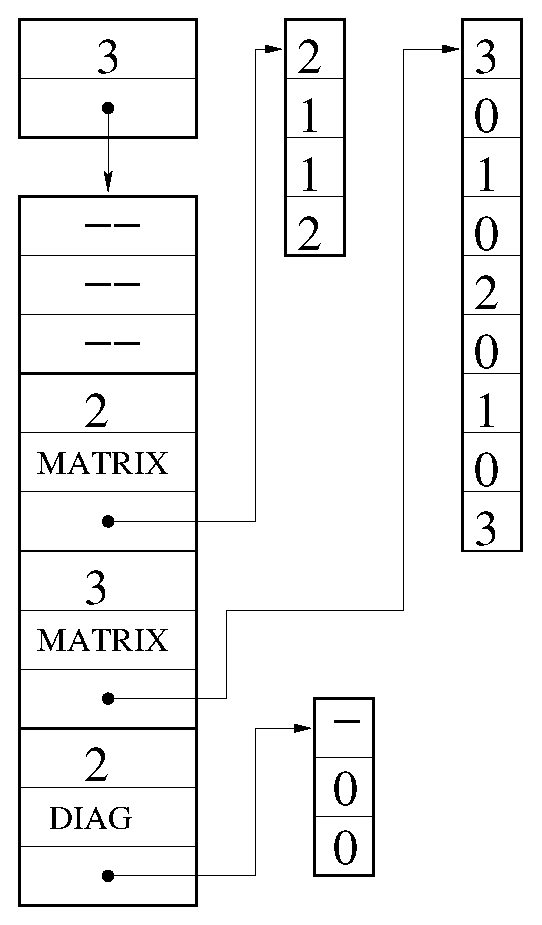
\includegraphics{cmat}}
\caption{The C matrix.}
\label{cmat}
\end{center}
\end{figure}

Figure \ref{constraints} shows the overall structure of the constraints.  There
is a vector of pointers to linked lists of constraint blocks.  The 0th entry
in this array is ignored.  Blocks that contain only zero entries are not
stored in the linked lists.  Figure \ref{a1block1} shows the detail
of the data structure for block 1 of the constraint matrix $A_{1}$.     

\begin{figure}
\begin{center}
\scalebox{0.5}{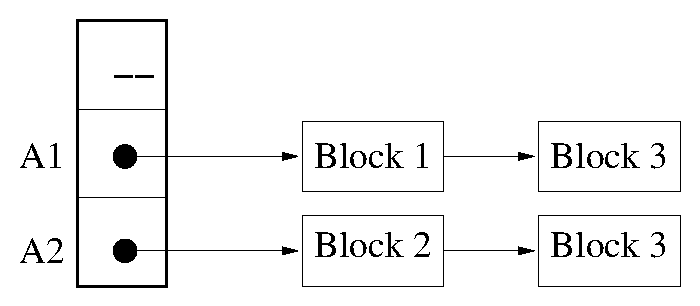
\includegraphics{constraints}}
\caption{The constraints.}
\label{constraints}
\end{center}
\end{figure}

\begin{figure}
\begin{center}
\scalebox{0.5}{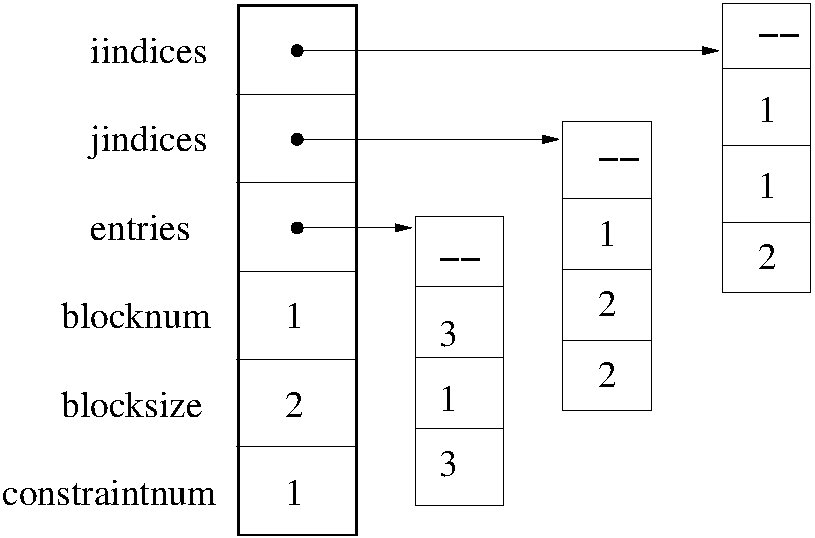
\includegraphics{a1block1}}
\caption{Block 1 of $A_{1}$.}
\label{a1block1}
\end{center}
\end{figure}

\clearpage

After solving the problem, the example program outputs the solution to 
prob.sol using the write\_sol() routine.  The output produced on 
different computers might vary because of floating point round--off
differences.  However, the following output is typical.

\begin{verbatim}
7.499999999674811235e-01 9.999999995736339464e-01 
1 1 1 1 2.500000018710683558e-01 
1 1 1 2 -2.500000000325189320e-01 
1 1 2 2 2.500000018710683558e-01 
1 2 1 1 6.895272851149165827e-10 
1 2 1 3 -4.263660251297748376e-10 
1 2 2 2 2.000000000263161049e+00 
1 2 3 3 1.999999999836795217e+00 
1 3 1 1 7.500000019361059422e-01 
1 3 2 2 1.000000001542258765e+00 
2 1 1 1 1.250000001467082567e-01 
2 1 1 2 1.249999992664581755e-01 
2 1 2 2 1.250000001467082567e-01 
2 2 1 1 6.666669670820890570e-01 
2 2 1 3 -4.518334811445142147e-07 
2 2 2 2 2.200629338637236883e-10 
2 2 3 3 2.200635108933231998e-10 
2 3 1 1 5.868341556035494699e-10 
2 3 2 2 4.401258478508541047e-10 
\end{verbatim}

The first line of the file gives the optimal y values.  The lines that
start with "1 " give the nonzero entries in the optimal Z matrix.  As in
the SDPA input file there are five numbers per line.  The first number
is the number of the matrix, where 1 is used for $Z$ and 2 is used
for $X$.  The second number specifies a block within the matrix.
The third and fourth numbers are the row and column within the block.
The final number is the actual value at the position in the block.
For example, 
\begin{verbatim}
2 2 1 3 -4.518334811445142147e-07 
\end{verbatim}
means that in the 1st row, third column of block 2 of the $X$ matrix, the
entry is $-4.518334811445142147\times 10^{-7}$. 
Since the matrices are symmetric, we only record
the entries in the upper triangle of the matrix.   The same entry will
also appear in row 3, column 1.  

So, the optimal solution to the example problem is (rounding the
numbers off to two or three digits)

\begin{equation}
y=\left[
\begin{array}{rr}
0.75 & 1.00 
\end{array}
\right]
\end{equation}

\begin{equation}
Z=\left[
\begin{array}{rrrrrrr}
 0.25 & -0.25 &   &   &   &   &    \\ 
 -0.25 & 0.25 &   &   &   &   &    \\ 
   &    & 0 & 0 & 0 &   &    \\ 
   &    & 0 & 2.00 & 0 &   &    \\ 
   &    & 0 & 0 & 2.00 &   &    \\ 
   &    &   &   &   & 0.75 &    \\ 
   &    &   &   &   &   & 1.00  \\ 
\end{array}
\right]
\end{equation}

\begin{equation}
X=\left[
\begin{array}{rrrrrrr}
 0.125 &  0.125 &   &   &   &   &    \\ 
 0.125 &  0.125 &   &   &   &   &    \\ 
   &    & 0.667 & 0 & 0 &   &    \\ 
   &    & 0 & 0 & 0 &   &    \\ 
   &    & 0 & 0 & 0 &   &    \\ 
   &    &   &   &   & 0 &    \\ 
   &    &   &   &   &   & 0  \\ 
\end{array}
\right]
\end{equation}

\subsection*{Storage Requirements}
CSDP requires storage for a number of block diagonal matrices of the same
form as $X$ and $Z$, as well as storage for the Schur complement system that
is Cholesky factored in each iteration.  For a problem with $m$ constraints
and block diagonal matrices with blocks of size $n_{1}$, $n_{2}$, $\dots$, 
$n_{s}$, CSDP requires approximately 
\begin{equation}
\mbox{Storage}=8(m^{2}+11(n_{1}^{2}+n_{2}^{2}+\ldots+n_{s}^{2}))
\end{equation}
bytes of storage.  This formula includes all of the two dimensional
arrays but leaves out the one dimensional vectors.  This formula also
excludes the storage required to store the constraint matrices, which
are assumed to be sparse.  In practice it is wise to allow for about
10\% to 20\% more storage to account for the excluded factors.

The parallel version of CSDP requires additional storage for work
matrices used by the routine that computes the Schur complement
matrix.  If the OpenMP maximum number of threads (typically the number
of processors on the system) is $p$, and $p>1$, then CSDP will
allocate an additional $16(p-1)n_{\mbox{max}}^{2}$
bytes of storage for workspace.

\subsection*{Calling The SDP Routine}
The routine has 11 parameters which include the problem data and an
initial solution.  The calling sequence for the sdp subroutine is:

\begin{verbatim}
int easy_sdp(n,k,C,a,constraints,constant_offset,pX,py,pZ,ppobj,pdobj)
   int n;                                 /* Dimension of X */
   int k;                                 /* # of constraints */
   struct blockmatrix C;                  /* C matrix */
   double *a;                             /* right hand side vector */
   struct constraintmatrix *constraints;  /* Constraints */
   double constant_offset;                /* added to objective */
   struct blockmatrix *pX;                /* X matrix */
   double **py;                           /* y vector */
   struct blockmatrix *pZ;                /* Z matrix */
   double *ppobj;                         /* Primal objective */
   double *pdobj;                         /* Dual objective */
\end{verbatim}
\subsection*{Input Parameters}
\begin{enumerate}
\item {\tt n}. This parameter gives the dimension of the X, C, and Z matrices.
\item {\tt k}. This parameter gives the number of constraints.
\item {\tt C}.  This parameter gives the $C$ matrix and implicitly defines 
the block structure of the block diagonal matrices.
\item {\tt a}.  This parameter gives the right hand side vector $a$.
\item {\tt constraints}.  This parameter specifies the problem constraints.
\item {\tt constant\_offset}.  This scalar is added to the primal and dual 
objective values.  
\item {\tt pX}.  On input, this parameter gives the initial primal solution $X$.
\item {\tt py}.  On input, this parameter gives the initial dual solution $y$.
\item {\tt pZ}.  On input, this parameter gives the initial dual solution $Z$.
\end{enumerate}
\subsection*{Output Parameters}
\begin{enumerate}
\item {\tt pX}.  On output this parameter gives the optimal primal solution $X$. 
\item {\tt py}.  On output, this parameter gives the optimal dual solution $y$.
\item {\tt pZ}.  On output, this parameter gives the optimal dual solution $Z$.
\item {\tt ppobj}.  On output, this parameter gives the optimal primal objective value.
\item {\tt pdobj}.  On output, this parameter gives the optimal dual objective value.
\end{enumerate}
\subsection*{Return Codes}
If CSDP succeeds in solving the problem to full accuracy, 
the {\tt easy\_sdp} routine will return 0.  
Otherwise, the {\tt easy\_sdp} routine will return a nonzero
return code.  In many cases, CSDP will have actually found a good 
solution that doesn't quite satisfy one of the termination criteria.
In particular, return code 3 is usually indicative of such a solution.
Whenever there is a nonzero return code, you should examine the return 
and the solution to see what happened.  
    
The nonzero return codes are
\begin{enumerate}
\item Success.  The problem is primal infeasible. 
\item Success.  The problem is dual infeasible.
\item Partial Success.  A solution has been found, but full accuracy was
not achieved.  One or more of primal infeasibility, dual infeasibility, 
or relative duality gap are larger than their tolerances, but by a factor
of less than 1000.
\item Failure.  Maximum iterations reached.
\item Failure.  Stuck at edge of primal feasibility.
\item Failure.  Stuck at edge of dual infeasibility.
\item Failure.  Lack of progress.
\item Failure.  X, Z, or O was singular.
\item Failure.  Detected NaN or Inf values.  
\end{enumerate}
\subsection*{The User Exit Routine}

By default, the {\tt easy\_sdp} routine stops when it has obtained a
solution in which the relative primal and dual infeasibilities and the
relative gap between the primal and dual objective values is less than
$1.0 \times 10^{-8}$.  There are situations in which you might want to
terminate the solution process before an optimal solution has been
found.  For example, in a cutting plane routine, you might want to
terminate the solution process as soon as a cutting plane has been
found.  If you would like to specify your own stopping criteria, you
can implement these in a user exit routine.

At each iteration of its algorithm, CSDP calls a routine named {\tt
user\_exit}.  CSDP passes the problem data and current solution to
this subroutine.  If {\tt user\_exit} returns 0, then CSDP continues.
However, if {\tt user\_exit} returns 1, then CSDP returns immediately
to the calling program.  The default routine supplied in the CSDP
library simply returns 0.  If CSDP is compiled 
with the ``-DUSESIGTERM'' flag, then default routine will also stop
the solution process whenever the process receives a TERM signal.
You can write your own routine and link it
with your program in place of the default user exit routine.

The calling sequence for the user exit routine is
\begin{verbatim}
int user_exit(n,k,C,a,dobj,pobj,constant_offset,constraints,X,y,Z,params)
   int n;                                 /* Dimension of X */
   int k;                                 /* # of constraints */
   struct blockmatrix C;                  /* C matrix */
   double *a;                             /* right hand side */
   double dobj;                           /* dual objective  */
   double pobj;                           /* primal objective */
   double constant_offset;                /* added to objective */ 
   struct constraintmatrix *constraints;  /* Constraints */
   struct blockmatrix X;                  /* primal solution */
   double *y;                             /* dual solution */
   struct blockmatrix Z;                  /* dual solution */
   struct paramstruc params;              /* parameters sdp called with */
\end{verbatim}
\subsection*{Finding an Initial Solution}
The CSDP library contains a routine for finding an initial solution to the
SDP problem.  Note that this routine allocates all storage required for the
initial solution.  The calling sequence for this routine is:

\begin{verbatim}
void initsoln(n,k,C,a,constraints,pX0,py0,pZ0)
   int n;                                  /* dimension of X */
   int k;                                  /* # of constraints */
   struct blockmatrix C;                   /* C matrix */
   double *a;                              /* right hand side vector */
   struct constraintmatrix *constraints;   /* constraints */
   struct blockmatrix *pX0;                /* Initial primal solution */
   double **py0;                           /* Initial dual solution */
   struct blockmatrix *pZ0;                /* Initial dual solution */
\end{verbatim}


\subsection*{Reading and Writing Problem Data}
The CSDP library contains routines for reading and writing SDP
problems and solutions in SDPA format. The routine {\tt write\_prob}
is used to write out an SDP problem in SDPA sparse format.  The
routine {\tt read\_prob} is used to read an SDP problem in from a
file.  The routine {\tt write\_sol} is used to write an SDP solution
to a file.  The routine {\tt read\_sol} is used to read a solution
from a file.

The calling sequence for {\tt write\_prob} is 

\begin{verbatim}
int write_prob(fname,n,k,C,a,constraints)
   char *fname;                          /* file to write */
   int n;                                /* Dimension of X */
   int k;                                /* # of constraints */
   struct blockmatrix C;                 /* The C matrix */
   double *a;                            /* The a vector */
   struct constraintmatrix *constraints; /* the constraints */
\end{verbatim}

The calling sequence for {\tt read\_prob} is:

\begin{verbatim} 
int read_prob(fname,pn,pk,pC,pa,pconstraints,printlevel)
   char *fname;                /* file to read  */
   int *pn;                    /* Dimension of X */
   int *pk;                    /* # of constraints */
   struct blockmatrix *pC;     /* The C matrix */
   double **pa;                /* The a vector */
   struct constraintmatrix **pconstraints;  /* The constraints */
   int printlevel;             /* =0 for no output, =1 for normal
                                  output, >1 for debugging */
\end{verbatim}
Note that the {\tt read\_prob} routine allocates all storage required
by the problem.  
 
The calling sequence for {\tt write\_sol} is 

\begin{verbatim}
int write_sol(fname,n,k,X,y,Z)
   char *fname;                     /* Name of the file to write to */
   int n;                           /* Dimension of X */
   int k;                           /* # of constraints */
   struct blockmatrix X;            /* Primal solution X */
   double *y;                       /* Dual vector y */
   struct blockmatrix Z;            /* Dual matrix Z */
\end{verbatim}
This routine returns 0 if successful and exits if it is unable to write
the solution file.  

The calling sequence for {\tt read\_sol} is 

\begin{verbatim}
int read_sol(fname,n,k,C,pX,py,pZ)
   char *fname;                     /* file to read */
   int n;                           /* dimension of X */
   int k;                           /* # of constraints */
   struct blockmatrix C;            /* The C matrix */
   struct blockmatrix *pX;          /* The X matrix */
   double **py;                     /* The y vector */
   struct blockmatrix *pZ;          /* The Z matrix */
\end{verbatim}
Note that {\tt read\_sol} allocates storage for $X$, $y$, and $Z$.  This
routine returns 0 when successful, and exits if it is unable to read
the solution file.  

\subsection*{Freeing Problem Memory}
The routine {\tt free\_prob} can be used to automatically 
free the memory allocated for a problem.  The calling sequence
for {\tt free\_prob} is

\begin{verbatim}
void free_prob(n,k,C,a,constraints,X,y,Z)
    int n;                                /* Dimension of X */
    int k;                                /* # of constraints */
    struct blockmatrix C;                 /* The C matrix */
    double *a;                            /* The a vector */
    struct constraintmatrix *constraints; /* the constraints */
    struct blockmatrix X;                 /* X matrix. */ 
    double *y;                            /* the y vector. */
    struct blockmatrix Z;                 /* Z matrix. */
\end{verbatim}

\bibliography{sdp}
 
\end{document}


